\textbf{Change this introduction to fit the final product!}
In this one year long project, we have collected results of a great number of materials with various structures and compositions. The initial experimentation was based on high-entropy silicides of the $Fe_2Si$ unit cell, created from the special quasi-random structure approach as described above. Despite the non-semiconducting character of this compound, we worked under the idea that the extraordinary properties that have been observed in high-entropy alloys through effects such as the cocktail effect, we could discover specific combinations of elements that would yield a semiconductor. In addition, the ratio between silicon atoms to metals allowed us to create nearly eqvimolar high-entropy alloys. 

Following this attempt, we transitioned into studying high-entropy silicides based on well known semiconducting 3d silicides such as $\beta-$\ch{FeSi2}, \ch{CrSi2} and \ch{MnSi_{1.75}}. The main outcome of this project is that for all 4 different starting silicides, we could only produce high-entropy silicides from one unit cell, furthermore in this cell only one specific compositions of elements was semiconducting. This was \ch{Cr_{0.25}Fe{0.25}Mn_{0.25}Ni_{0.25})Si2}, here-in CFMN, in the $\beta-$ \ch{FeSi2} crystal structure.  

This section will be structured in the following manner, firstly we will investigate the CFMN (fesi2) compound and various permutations of the composition. Thereafter we will look at other possible compositions of fesi2 based high-entropy silicides, and lastly test the CFMN composition in other crystal symmetries. In final we will present an overview of the complete study and the various compounds that have been investigated in order to propose promising directions and guideline future research directions in this field. In this way, we aim to understand the uniqe properties of CFMN (fesi2) and why this particular compound is semiconducting compared to the other testes structures in this project. Properties we will cover is the overall stability by total energy and corresponding enthalpy of formation, the magnetic properties and which elements contribute to the magnetism. But in majority, we will look at the band gap and related properties, as this is the main motivation and distinction of the study.

\textbf{Add figure DOS FeSi2?}


\chapter{The results of equimolar \ch{(CrFeMnNi)Si2} in the $\beta-$\ch{FeSi2} structure}
\label{sec:equi}

$\beta-FeSi_2$ in the orthorombic cmce crystal lattice is a well known semiconductor with an experimentally measured band gap of around 0.85 ev at room temperature \cite{PhysRevB.58.10389}, the nature of the band gap is under debate, all though most ab inito studies point to an indirect gap, experimental work indicate a direct gap. From our calculations we find an indirect band gap close to 0.65 eV with PBE, compared for example materials project's listed value of 0.698 eV with the same functional. Moreover in agreement with the calculations of materials project we discover that bulk $\beta-$ \ch{FeSi2} is diamagnetic. Finally, the enthalpy of formation of this compound is calculated as $-18.6583 eV$.

The high-entropy alloys generated from the \ch{FeSi2} unit cell alloys can be seen in figure 6.1. The supercells consist of 48 atoms each, in which the 16 iron sites is occupied equimolarly between Cr, Fe, Mn, and Ni, and the 32 silicon sites is as before occupied by silicon. Bellow in table 7.1 we list the enthalpy of formation ($\Delta H^0$) in addition to the total energy per atom (Toten), final magnetic moment per atom (Mag), and the band gap $E_G$, for the five distinct SQSs plus the mean and standard deviation of the set. For simplicity, we denote the 5 supercells as A, B, C, D and E respectively.

\begin{table}[H]
\centering
\begin{tabular}{@{}cccc@{}}
\toprule
Structure  & Toten (eV) & Mag ($\mu_B$) & Band gap (eV) \\ \midrule
\textbf{A} & −6,6080                & 0.0833                    & 0.0280        \\
\textbf{B} & −6,6138                & 0.0833                    & 0.0523        \\
\textbf{C} & −6,6063                & 0.0834                    & 0.0344        \\
\textbf{D} & −6,6155                & 0.0833                    & 0             \\
\textbf{E} & −6,6089                & 0.0833                    & 0.0495        \\ \midrule
\textbf{Mean} & -6.6105 & 0.0833 & 0.0328    \\
\textbf{Std} & 0.0039 &  0.0000 &  0.0210 \\
\textbf{$\Delta H_{mean}^0$} & -11.5000 eV & - & - \\ \bottomrule
\end{tabular}
\caption{Total energy per atom, final magnetic moment, band gap (GGA) and formation enthalpy of $Cr_4Fe_4Mn_4Ni_4Si_{32}$ SQSs based on $FeSi_2$}
\label{table:fesi2_summary}
\end{table}  

From a first glance it's a clear distinction between the SQSs, especially in terms of the band gap and less so for the total magnetic moment. On the grounds of the total energy we note that the most stable supercell is SQS D, and reversely the least stable is SQS A. The band gaps listed in table 7.1 point to that the large majority of the SQSs are narrow-gap semiconductors in the range 0.028 - 0.052 eV, but the utmost stable configuration D does not exhibit any finite band gap.

In terms of the magnetism we see that contrary to the bulk \ch{FeSi2} compound that this alloy is magnetic. Investigating the local magnetic moments of SQS D we discover that the ferromagnetic iron and nickel contain very small moments and non-existent in Ni.On the other hand the anti-ferromagnetic elements chromium and manganese contain large magnetic moments. In section 2.2 we provided several examples where Cr was known to reduce the saturation magnetization of high-entropy alloys. For example in the ferromagnetic HEA CoFeMnNiX, X = Al, Cr, Ga, Sn, studied in \cite{ZUO201710}. Mn had minimal impact on the magnetism and favoured the ferromagnetic phase, meanwhile addition of Cr pushed the material to a paramagnetic phase. Likewise in the eqvimolar system of \ch{CrMnFeCoNi} \cite{PhysRevB.96.014437}, the local magnetic moment of Cr was found to align antiferromagnetic, and the ferromagnetic character was attributed to local magnetic moments of Fe and Mn. The odd magnetic properties experienced in this alloy can be related to several factors. Firstly are the limitations mentioned previously about about both DFT and special quasi-random structures to model magnetic and particularly paramagnetic materials. Further the magnetic investigation and focus in this project have been very superficial with only considering non-spin polarized calculations or co-linear spin polarization, thus the phases in-between have been neglected. Lastly only the the ground state, ie 0K have been studied. Hence the reported magnetic properties should be taken with a grain of salt and are intended for subsequent studies focused on the magnetic properties of this alloy especially at non-zero temperatures. 

\section{The band gap}

\begin{figure}[H]
	\centering
	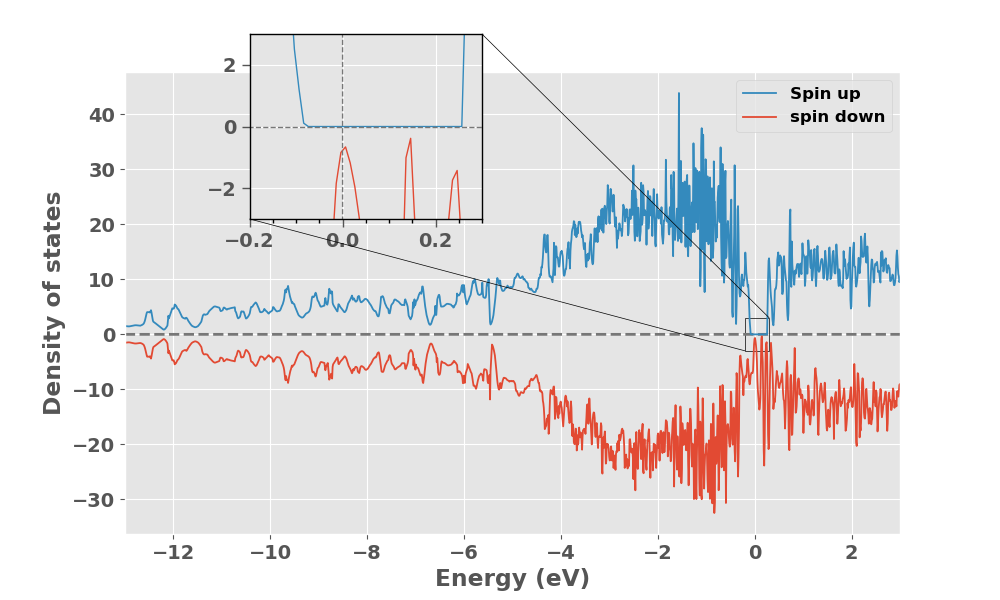
\includegraphics[width=.8\textwidth]{results/fesi2/D_TDOS.png}
	\caption{Density of states of SQS D \ch{(CrFeMnNi)Si2} with PBE.}
\end{figure}

\begin{figure}[H]
\centering
	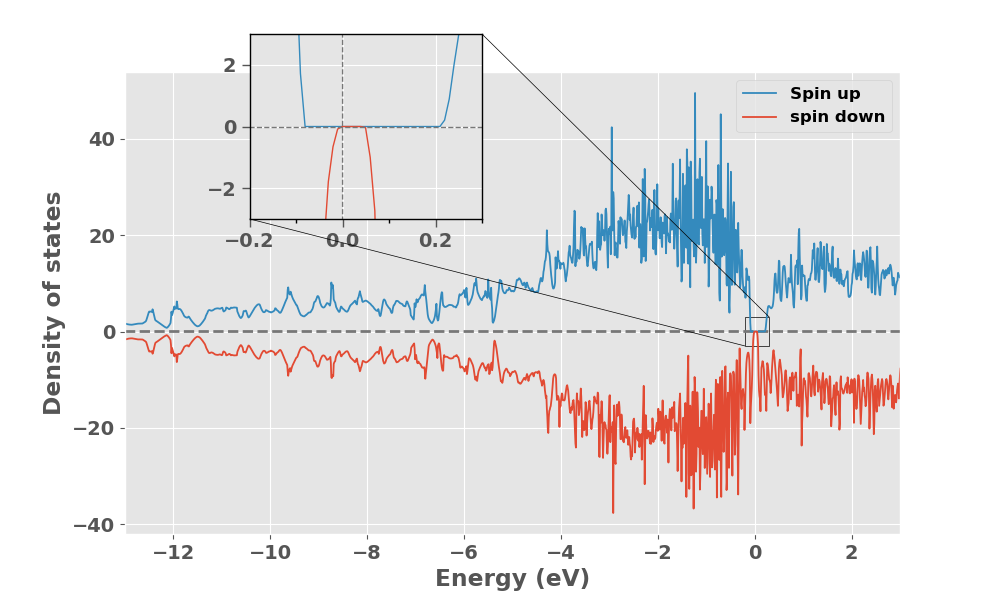
\includegraphics[width=.8\textwidth]{results/fesi2/B_TDOS.png}
	\caption{Density of states of SQS B \ch{(CrFeMnNi)Si2} with PBE.}
\end{figure}  

Above we plot the electronic density of states of SQS D and B from calculations with the PBE GGA functional. These supercells and corresponding properties are emphasized due to the relative stability in the set. Being the most stable means it's the most representative structure of the potentially "real" material, and hence so are the properties of that SQS. From the DOS in figure 7.1 we discover that the structure is in fact a half-metal with a band gap around 0.3 eV in the spin up channel and a metal in spin down. The exact value of the band gap in spin up is calculated from the range of energies corresponding 0 density of states around $E_F$, ie $ 0.2 eV - (-0.1 eV) = 0.3 eV$. Following the total band gap of the solid is determined by the minimum range of energies from both spins, which in this case is 0 from the spin down DOS. Since these values are calculated by the density of states they will be denoted as $E_G ^\text{up, dos}$ and $E_G ^\text{dw, dos}$ to indicate the spin direction. By the same mannerism we can see from figure 7.2 that the second utmost stable SQS (B) clearly contain finite values of both $E_G ^\text{up, dos}$ and $E_G ^\text{dw, dos}$. Similar figures can be seen for SQS A, C, and E in appendix ..,  all respective spin dependent band gaps is listed below in table 7.2. 

These values are determined from the calculated eigenvalues, and hence will be referenced to as $E_G ^\text{up, eigen}$ and $E_G ^\text{dw, eigen}$. This value is found by subtracting the highest energy eigenvalue in the valence band from the lowest energy eigenvalue in the conduction band. Across all five SQSs we observe in accordance with the magnetic property a distinction between spins where $E_G ^\text{up} > E_G ^\text{dw}$.
 
\begin{table}[H]
\centering
\begin{tabular}{@{}cccc@{}}
\toprule
SQS  & $E_G ^\text{up, eigen}$ (meV) & $E_G ^\text{dw, eigen}$ (meV) & $E_G ^\text{t, eigen}$ (meV)   \\ \midrule
\textbf{A} & 81.4  & 52.2   & 28.1 \\
\textbf{B} & 293  & 52.2    & 52.2 \\
\textbf{C} & 236  & 34.3    & 34.3 \\
\textbf{D} & 339  & 0.00    & 0.00      \\
\textbf{E} & 308  & 50.0    & 50.0 \\ \bottomrule
\end{tabular}
\caption{Band gap (eV) with PBE in spin up and spin down channels of CFMN (fesi2) SQSs}
\end{table}
  
Alike the bulk material, these gaps are indirect. It would have been instructive to visualize and analyze the energy bands by plotting the band structure. Unfortunately this is neither simple to perform or interpret in large supercells consisting of several elements and a large number of energy bands. One solution is to do band-unfolding, but given the complex structure and implementation of the special quasi-random structures method in VASP this proved too challenging for the scope of this project. 

 
\textbf{ \\ Visualize the eigenvalues ??}

A key point regarding the band structure of SQS D is the presence of defect states. In this structure the highest occupied conduction band is 128 for spin up states and band 124 in spin down, thus a difference of 4 bands between spins. For the spin down states we find that the highest energy conduction band, ie 124 have states with occupancy both slightly bellow 1.00 and above at several k-points. Likewise the lowest energy valence band (124) have partially filled states above 0.00 and bellow. The case of occupancy either above or bellow completely full or completely empty is simply a numerical inaccuracy well-known to calculations that apply the Tetrahedron method with Bloch corrections and have no real impact on the results. The second case where we have partially filled eigenstates in the conduction band and not completely filled states is a familiar term in random alloys \cite{PhysRevLett.104.236403} in which the forbidden energy gap is contaminated by defect states. To further study this effect we introduce $E_G ^\text{eigen}(occ)$ to represent the band gap calculated at a cut-off occupancy in the eigenvalues such that $E_G ^\text{eigen}(0.99)$ only consider eigenstates with occupancy above 0.99 as filled. Equivalently $E_G ^\text{eigen}(0.01)$ only consider eigenstates with occupancy less than 0.01 as empty. By utilizing this parameter we can effectively study the band gap in relation to the defect states. Applying this to SQS D we get the results listed below in table .., keep in mind that $E_G ^\text{up, eigen}$ is constant from that the defect states are only present in the spin down channel. Moving further results listed without specifying $occ$ is equivalent to $occ = 0.5, 0.5$.

\begin{table}[H]
\centering
\begin{tabular}{@{}ccccc@{}}
\toprule
Occ (full)          & Occ (empty)      & $E_G ^\text{up, eigen}$ (meV)  & $E_G ^\text{dw, eigen}$ (meV) & $E_G ^\text{t, eigen}$ (meV) \\ \midrule
0.9                 & 0.1              & 339 & 0    & 0     \\
0.95                & 0.05             & 339 & 21.0 & 21.0  \\
0.99                & 0.01             & 339 & 49.6 & 49.6  \\
0.999               & 0.001            & 339 & 73.3 & 73.3  \\
\textgreater 0.9999 & \textless 0.0001 & 339 & 85.7 & 85.7  \\ \bottomrule
\end{tabular}
\end{table}


\newpage
\section{Local and projected density of states}
  
\begin{figure}[H]
	\centering
	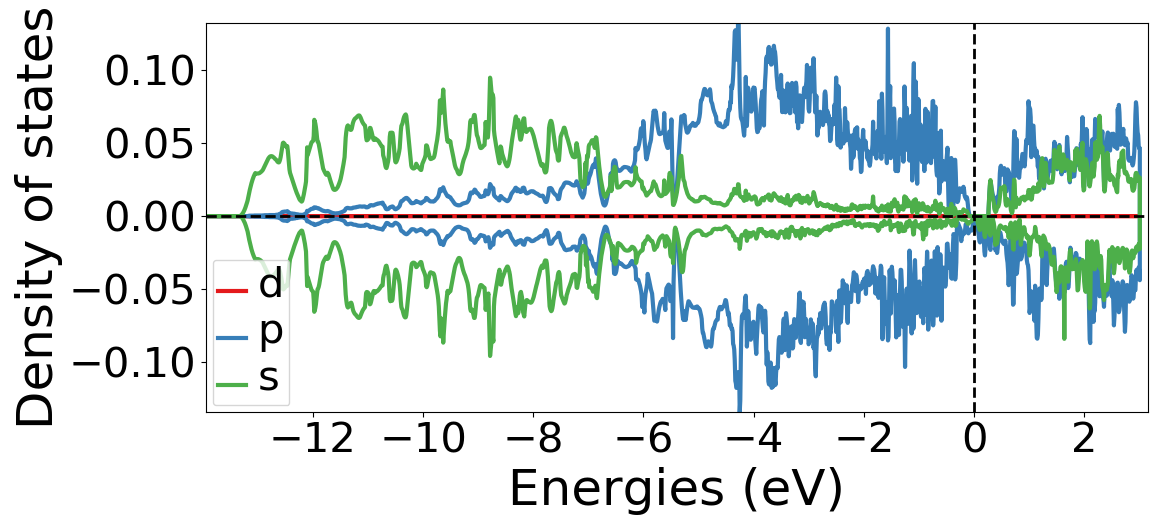
\includegraphics[width=.7\textwidth]{results/fesi2/D_LDOS_Si.png}
	\caption{Local density of states of Si (SQS D)}
\end{figure} 

\begin{figure}[H]
	\centering
	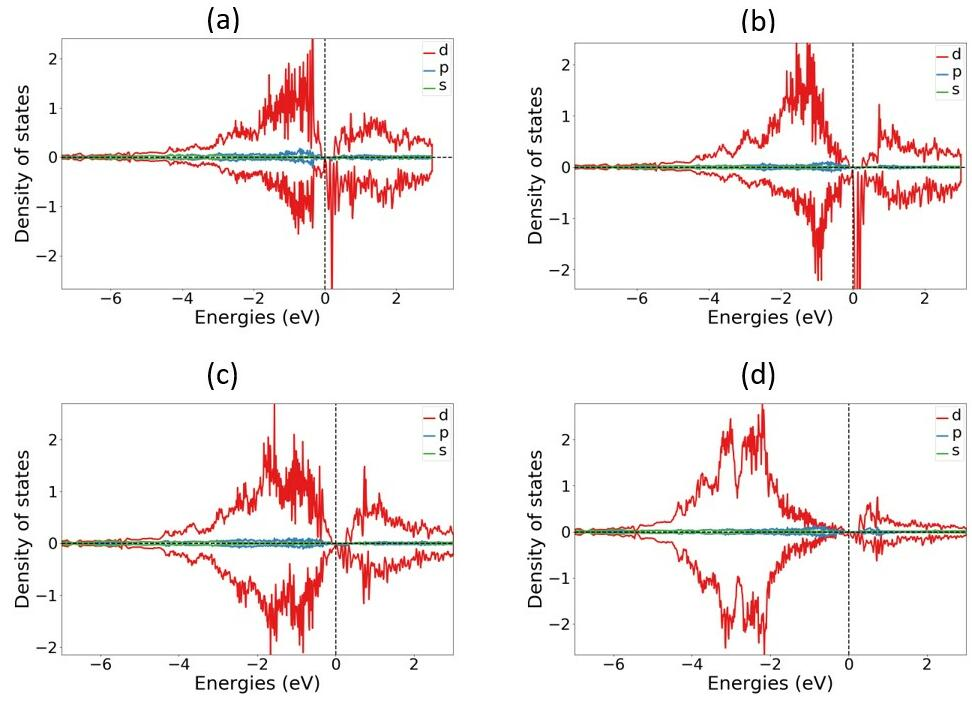
\includegraphics[width=\textwidth]{results/fesi2/D_LDOS.jpeg}
	\caption{Local density of states of (a) Cr, (b) Mn, (c) Fe, (d) Ni in SQS D.}
\end{figure}   
  
In the local density of states plotted in figure 7.3 we see that the s-electrons in Si occupy states in the lower energy regions and p electrons at slightly elevated energies closer to the Fermi energy, above $E_F$ states are occupied by both s and p electrons almost equally. Further, the local density of states of the transition metals chromium, manganese, iron and nickel in SQS D is displayed bellow in figure 7.4. In spin down, manganese is most dominant especially above $E_F$, but also bellow $E_F$. Likewise chromium show a strong presence above the Fermi energy in spin down. Both iron an Nicel show largest contribution at energies further from the Fermi energy, most notably bellow $E_F$. In the spin up channel we see a similar trend where chromium lie closest to $E_F$ followed by manganese then iron and lastly nickel at the lowest energies. Another interesting observation is that the the LDOS of iron and nickel is much more symmetric between spins, than Cr and Mn. Comparing to the LDOS of iron and silicon in bulk $\beta-$ \ch{FeSi2} \cite{doi:10.1063/1.346415} we find good agreement for both Fe and Si in this alloy .

\begin{figure}[H]
	\centering
	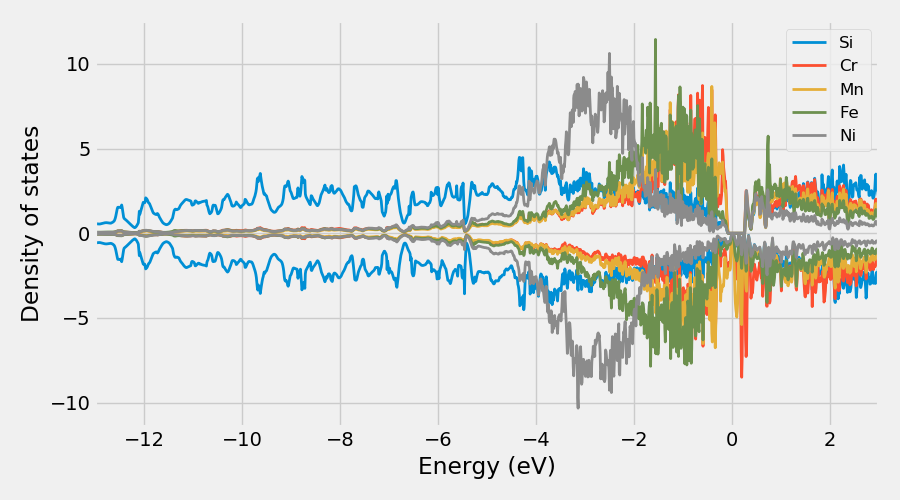
\includegraphics[width=.8\textwidth]{results/fesi2/D_PDOS.png}
	\caption{Projected density of states SQS D CFMN (fesi2) from PBE calculation}
\end{figure} 

Moreover the relative positions and interplay between 3d elements and silicon as shown in the projected density of states (figure 7.5) is in good agreement with observed trends in simpler Si-rich transition metal silicides \cite{lange1997electronic}. The electronic structure tends to be dominated by TM d electrons, and the valence band density of states are filled by non-bonding d states near $E_F$. The p-d hybridization between Si and TM elements typically fall about 6 eV bellow $E_F$ and Si $s$ states about 10 eV bellow. In our case we find that the Si states are pushed up closer to the fermi energy by random alloying of various 3d elements.    

  
\begin{figure}[H]
	\centering
	\begin{subfigure}{.45\textwidth}
			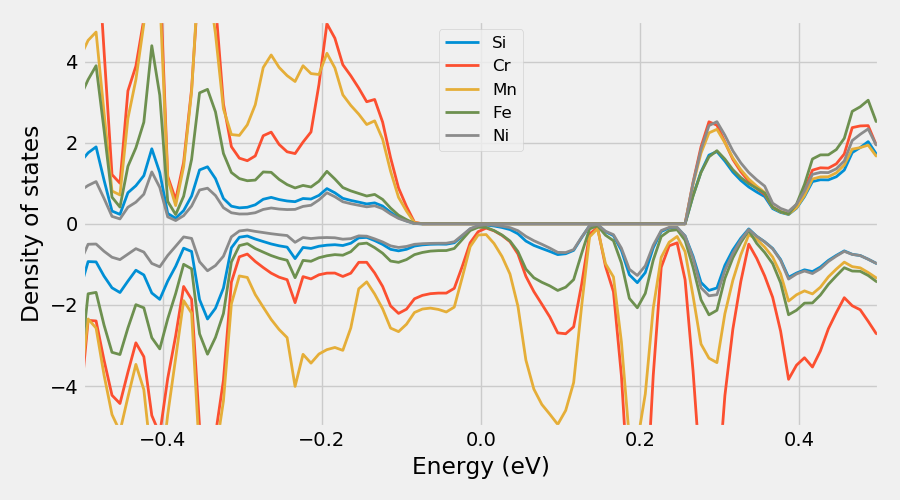
\includegraphics[width=\textwidth]{results/fesi2/D_PDOS_Ef.png}
			\caption{SQS D}		
	\end{subfigure}
	\hspace{0.5cm}
	\begin{subfigure}{.45\textwidth}
		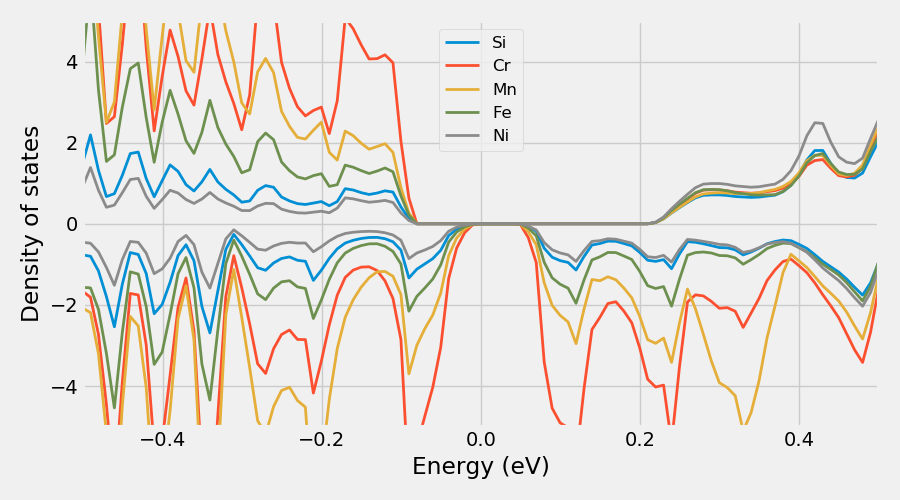
\includegraphics[width=\textwidth]{results/fesi2/B_PDOS_Ef.png}
		\caption{SQS B}		
	\end{subfigure}
	\caption{Projected density of states of SQS D and B around $E_F$}
\end{figure}

Above we have included the PDOS of SQS D and B but focused around $E_F$, from these figures we find that the spin down channel in D contain a more dominant presence of manganese especially, and some chromium as compared to the semiconducting SQS B.  

\section{Results from SCAN and HSE06 functionals}
As expressed previously in this work we invoke 3 level of depths GGA (PBE), meta-GGA (SCAN) and hybrid functional (HSE06) to determine the band gap of the SQSs. These results are showcased in table 7.3 for all five SQSs. Note that the eigen/dos and $occ$ parameters mentioned previously have been neglected as we only include the band gaps from default parameters that are in agreement between the density of states and eigenvalues.
 
\begin{table}[H]
\centering
\begin{tabular}{@{}ccccc@{}}
\toprule
SQS & XC-functional  & $E_G ^\text{up}$ (eV) & $E_G ^\text{dw}$ (eV) & $E_G ^\text{t}$ (eV) \\ \midrule
\multicolumn{1}{c|}{\multirow{3}{*}{\textbf{A}}}     & PBE & 0.0815                & 0.0521                  & 0.0281              \\
\multicolumn{1}{c|}{}                                & SCAN & 0                 & 0                  & 0           \\
\multicolumn{1}{c|}{}                                & HSE06 & 0.7084                & 0.0261                  & 0.0261                   \\ \midrule
\multicolumn{1}{c|}{\multirow{3}{*}{\textbf{B}}}     & PBE &  0.2932                & 0.0523                  & 0.0523              \\
\multicolumn{1}{c|}{}                                & SCAN & 0.1470                & 0.0890                  & 0.0890                  \\
\multicolumn{1}{c|}{}                                & HSE06 & 0.2855                & 0.1819                  & 0.1819                        \\ \midrule
\multicolumn{1}{c|}{\multirow{3}{*}{\textbf{C}}}     & PBE & 0.2355                & 0.0343                  & 0.0343              \\
\multicolumn{1}{c|}{}                                & SCAN & 0.0690                & 0.1124                  & 0.1124                   \\
\multicolumn{1}{c|}{}                                & HSE06 & 0.1744                & 0.0328                  & 0.0196                   \\ \midrule
\multicolumn{1}{c|}{\multirow{3}{*}{\textbf{D}}}     & PBE & 0.3386                & 0                       & 0                   \\
\multicolumn{1}{c|}{}                                & SCAN & 0                & 0.1086                  & 0                   \\
\multicolumn{1}{c|}{}                                & HSE06 & 0.3780                & 0                  & 0.          \\ \midrule
\multicolumn{1}{c|}{\multirow{3}{*}{\textbf{E}}}     & PBE & 0.3078                & 0.0495                  & 0.0495              \\
\multicolumn{1}{c|}{}                                & SCAN & 0.1540                & 0.1112                  & 0.1048                      \\
\multicolumn{1}{c|}{}                                & HSE06 & 0.5476                & 0.0133                  & 0.0133                   \\ \bottomrule
\end{tabular}
\caption{Total and spin band gap (eV) for 5 SQSs of \ch{(CrFeMnSi)2} with PBE, SCAN and HSE06}
\end{table}

Aside SQS A, all 3 functionals agree on the presence of the band gap, but the exact size of the band gap is under debate. We report the largest total band gap to be associated with the SCAN functional, compared to PBE this is expected considering the factors mentioned in section .. about the limitations of generalized gradient approximations. In contrast, by the same argument we would not expect that par SQS B, to find the overall lowest band gaps from the well-proven hybrid functional HSE06. Nevertheless we observe generally good agreement between PBE and HSE06 calculations, with both producing large $E_G ^\text{up}$ and small or zero in the case of SQS D $E_G ^\text{dw}$. In contrast as illustrated in figure 7.7 for SQS E (a + b) and D (c + d), SCAN enlarge the spin down value and decrease the spin up band gap in E and B, and further reverse the spin polarization of the band gap in SQSs C and D. Regarding SQS A, we find that the SCAN result suffers from defect states as was described previously for D, neglecting said states yield $E_\text{G, SCAN} ^{up, eigen}(0.99, 0.01) = 0.0316$ eV and $E_\text{G, SCAN} ^{dw, eigen}(0.99, 0.01) = 0.0531$ eV resulting in a total gap of 0.0316 eV. Comparing to table 7.3 this appears to be in better agreement with particularly PBE, still however we find also here the same inverse spin polarization with SCAN.  
 
\begin{figure}[H]
	\begin{subfigure}{.5\textwidth}
		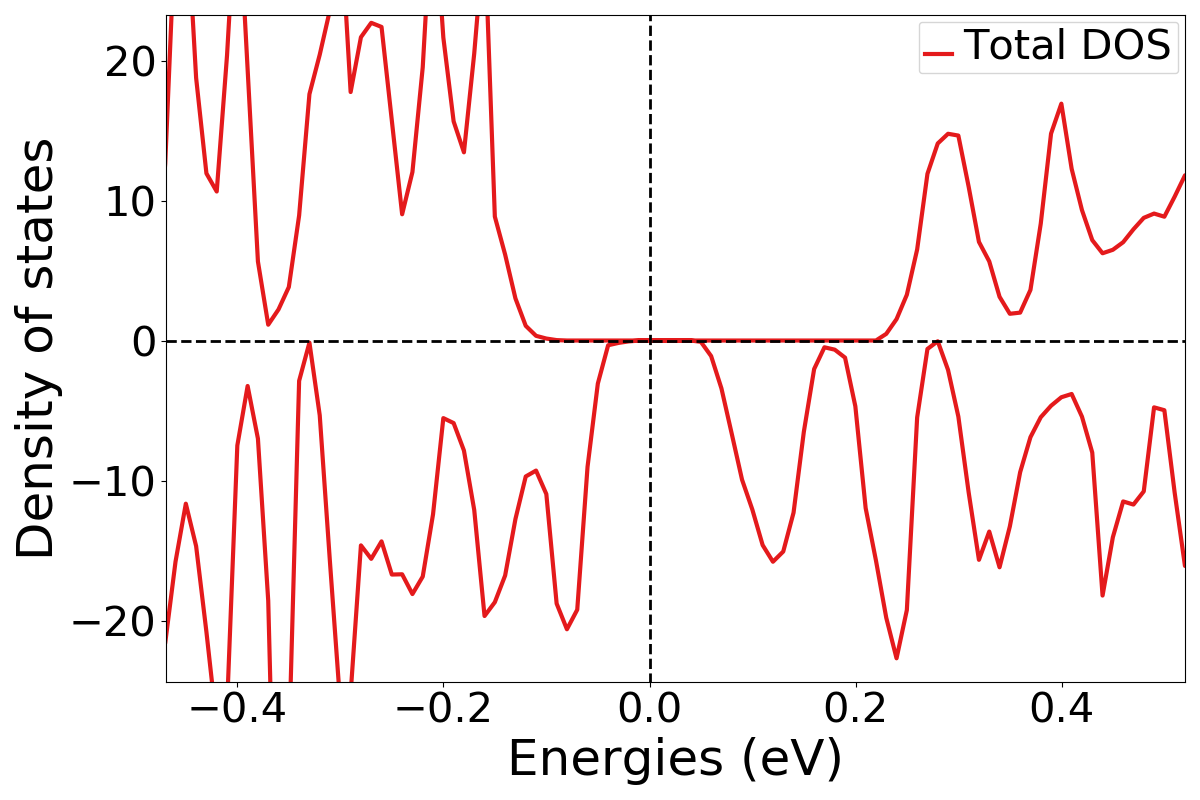
\includegraphics[width=\textwidth]{results/fesi2/E_DOS_pbe.png}
		\caption{SQS E PBE}
	\end{subfigure}
	\begin{subfigure}{.5\textwidth}
		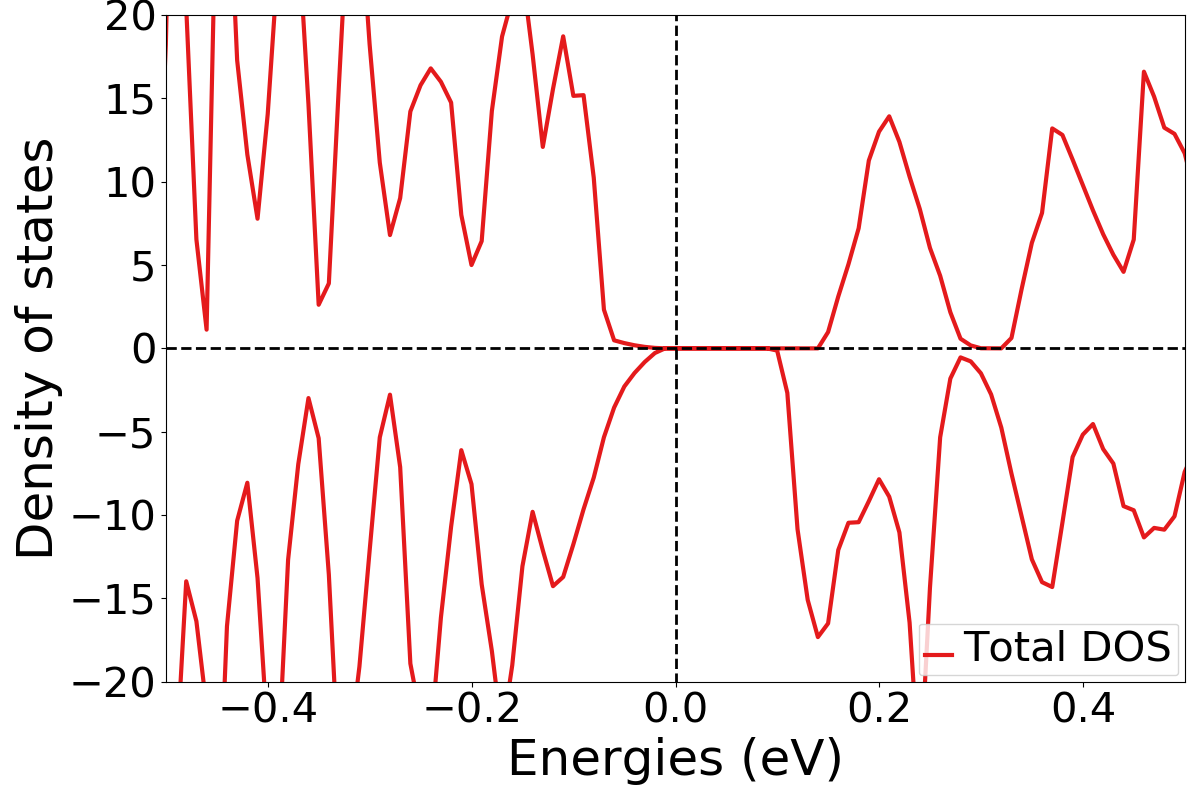
\includegraphics[width=\textwidth]{results/fesi2/E_DOS_scan.png}
		\caption{SQS E SCAN}
	\end{subfigure}
	\begin{subfigure}{.5\textwidth}
		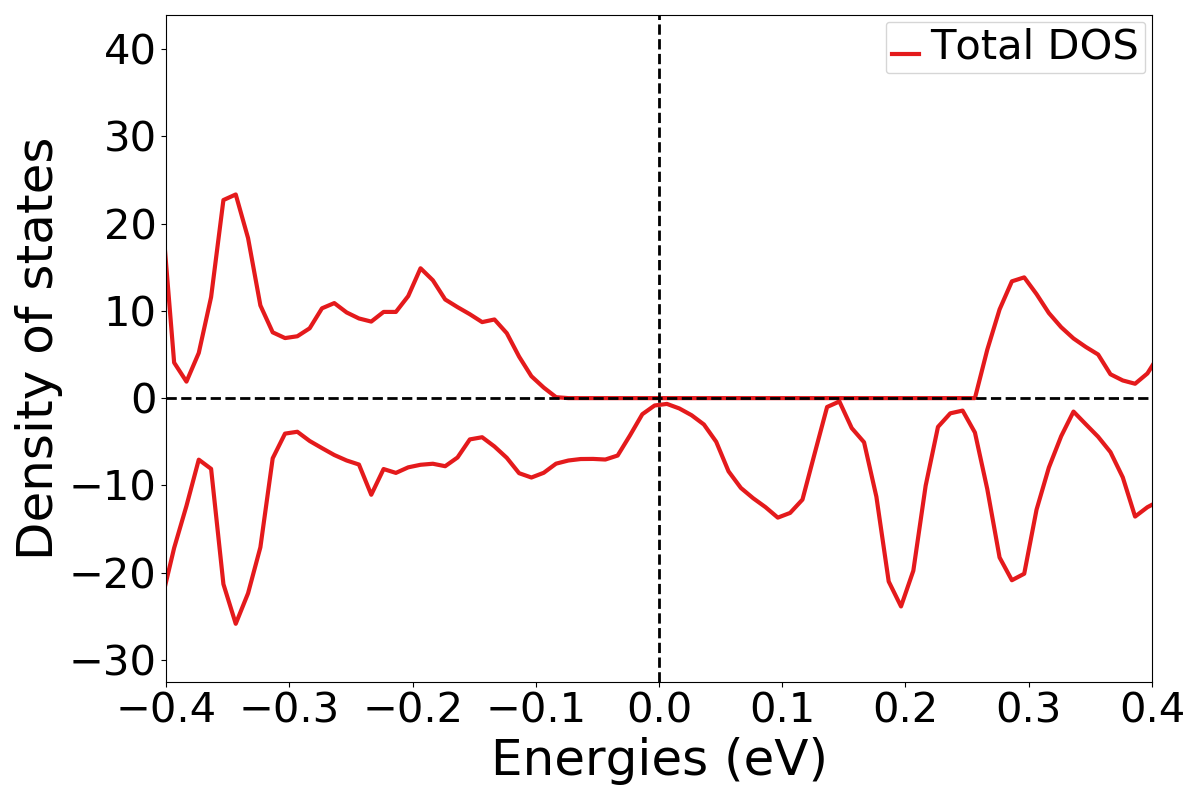
\includegraphics[width=\textwidth]{results/fesi2/D_DOS_pbe.png}
		\caption{SQS D PBE}
	\end{subfigure}
	\begin{subfigure}{.5\textwidth}
		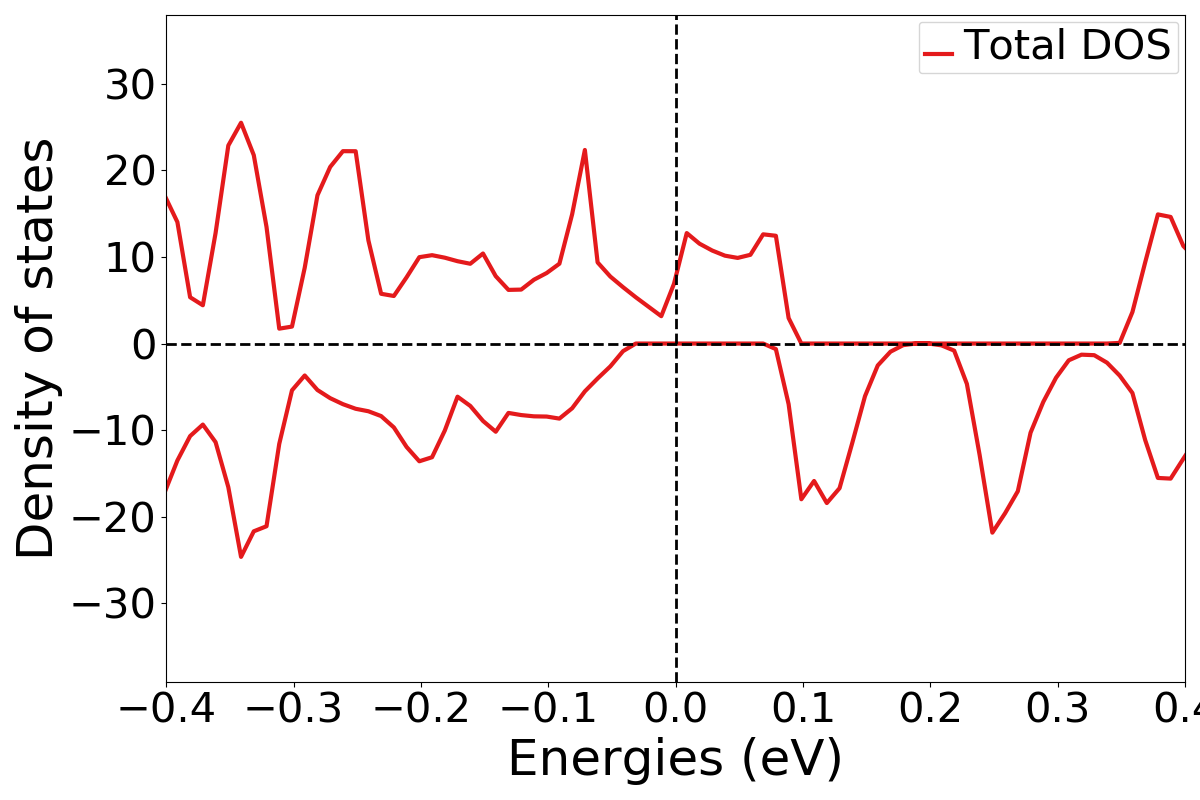
\includegraphics[width=\textwidth]{results/fesi2/D_DOS_scan.png}
		\caption{SQS D SCAN}
	\end{subfigure}
	\caption{Density of states illustrating the band gaps from PBE and SCAN calculations for SQS E and D.}
\end{figure}


As stated above, HSE06 and PBE calculations yield mostly similar characteristics of the band gap. Looking at the spin dependent band gaps however it's clear that HSE06 in show large deviation to PBE, for example enlarged values in $E_\text{G, A} ^{up}$, $E_\text{G, B} ^{dw}$, $E_\text{G, E} ^{up}$, or reduced values in $E_\text{G, A} ^{dw}$, $E_\text{G, E} ^{dw}$. And in other cases find nearly identical values to PBE as in $E_\text{G, B} ^{up}$ and $E_\text{G, C} ^{dw}$, or in SQS D that find excellent agreement in both spins. Generally we find that utilizing the HSE06 functional for these structures result in comparative or enlarged band gaps in spin up and lower values in spin down, with the exception of SQS B where HSE06 predicts a sizable band gap in both spins. Analog to the other cases, the 0 gap in D from HSE06 originates from defect states in the band structure, we get a band gap $E_\text{G, HSE06} ^{dw, eigen}(0.99, 0.01) = 0.2665$ eV from increasing the cutoff occupancy.
   
\begin{figure}[H]
	\centering	
	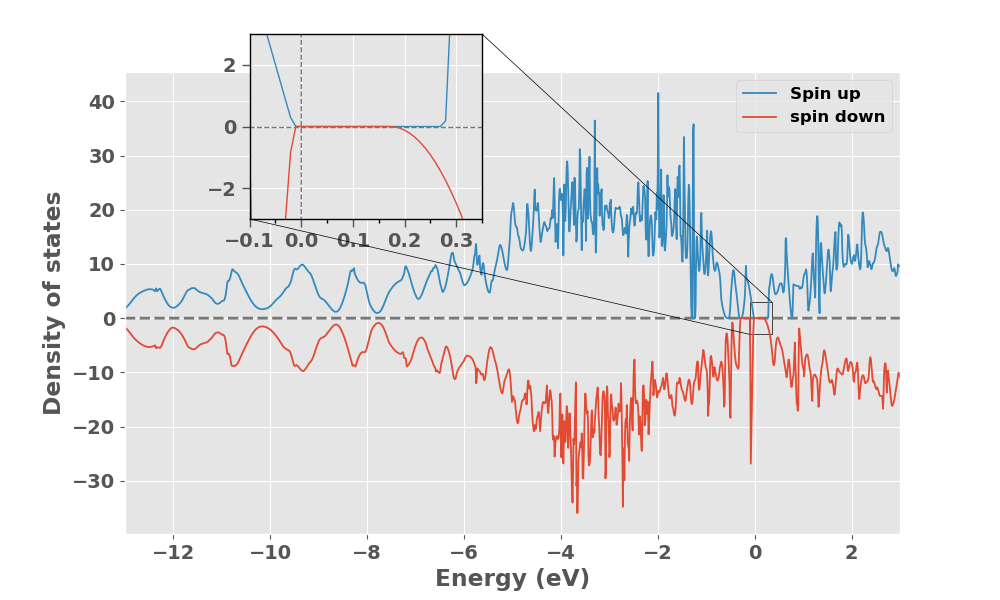
\includegraphics[width=\textwidth]{results/fesi2/B_TDOS_hse06.png}
	\caption{Density of states of SQS B with HSE06}
\end{figure}
 
The hybrid functional as expressed in section .. is computationally demanding to implement, in figure .. we show the computational cost in terms CPU-hours between PBE, SCAN and HSE06. One of the reasons behind the large cost of HSE06 is that we had to perform two subsequent calculations, firstly with Gaussian smearing and then secondly with TBC reapplying the calculated charge density. Nevertheless the CPU time of the first HSE06 calculation is still significantly greater than that of meta-GGA and GGA. Moreover the HSE06 calculations was performed with halve the number of k-points to PBE and SCAN in order to reach electronic convergence. Thus a completely justified comparison would contain even greater differences. 

\begin{figure}[H]
\centering
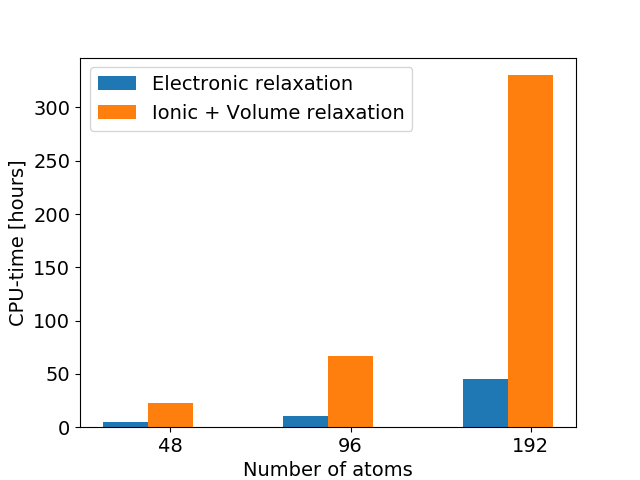
\includegraphics[width=.7\textwidth]{results/SQS_time.png}
\caption{Something}
\end{figure}

The narrow mesh of k-points in HSE06 calculations is an important factor to mention in relation to the HSE06 band gaps, that could lead to artificially exaggerated band gaps as the low density of k-points could fail to encapsulate the exact minimum transition between the valence band and conduction band. As seen in table 7.4 below the band gap is found between differing k-points from applying the 3 distinct functionals in SQS B (same in other SQSs).

\begin{table}[H]
\centering
\begin{tabular}{@{}cc@{}}
\toprule
XC-functional & VB $\rightarrow$ CB (k-point)                              \\ \midrule
PBE           & (0.250,0.000,0.250) $\rightarrow$ (0.000,0.000,0.000)  \\
SCAN          & (0.250,0.000,0.250) $\rightarrow$ (0.000,0.333,0.000)  \\
HSE06         & (0.500,0.000,0.000) $\rightarrow$ (0.000,0.000,0.000) \\ \bottomrule
\end{tabular}
\caption{Minimum gap between k-point in valence band (VB) and conduction band (CB) in SQS B from PBE, SCAN and HSE06}
\end{table}

The most concerning factor is that the highest energy k-point in the valence band from PBE calculations (0.250, 0.000, 0.250) is not considered in the HSE06 calculation with the narrow grid of 2x2x2 k-points. Thus one may suspect that the HSE06 calculation fails to locate the minimum transition. With a lack of an experimental baseline this becomes an important factor to consider primarily in the cases where the HSE06 functional predicts much greater values than PBE, such as $E_\text{G, A} ^{up}$ and $E_\text{G, B} ^{dw}$. Both PBE and SCAN have known limitations for 3d magnetic systems, on the other hand the sole drawback of the HSE06 functional is the computational demand which makes for possible errors from the methods one must employ to converge the calculations, such as lesser k-points. 

\newpage
\begin{landscape}
\begin{table}[H]
\centering
\begin{tabular}{@{}cccccccc@{}}
\toprule
SQS                                     & Smearing         & $E_\text{G} ^{up, eigen}(0.5)$ & $E_\text{G} ^{dw, eigen}(0.5)$ & $E_\text{G} ^{up, eigen}(0.01)$ & $E_\text{G} ^{dw, eigen}(0.01)$ & $E_\text{G} ^{t, eigen}(0.5)$ & $E_\text{G} ^{t, eigen}(0.01)$ \\ \midrule
\multicolumn{1}{c|}{\multirow{3}{*}{A}} & Gaussian (0.05 eV)  & 0.7837   & 0.1493   & -        & 0.2984   & 0.1493 & 0.2984  \\
\multicolumn{1}{c|}{}                   & Gaussian (0.005 eV) & 0.2117   & 0.1013   & -        & -        & 0.1013 & -       \\
\multicolumn{1}{c|}{}                   & TBC              & 0.7084   & 0.0261   & -        & -        & 0.0261 & -       \\ \midrule
\multicolumn{1}{c|}{\multirow{3}{*}{B}} & Gaussian (0.05 eV)  & 0.2783   & 0.1702   & 0.2988   & 0.3136   & 0.1506 & 0.2979  \\
\multicolumn{1}{c|}{}                   & Gaussian (0.005 eV) & 0.2838   & 0.1823   & -        & -        & 0.1801 & -       \\
\multicolumn{1}{c|}{}                   & TBC              & 0.2855   & 0.1819   & -        & -        & 0.1807 & -       \\ \midrule
\multicolumn{1}{c|}{\multirow{3}{*}{C}} & Gaussian (0.05 eV)  & 0.1078   & 0.1066   & 0.2405   & 0.1839   & 0.0650 & 0.1839  \\
\multicolumn{1}{c|}{}                   & Gaussian (0.005 eV) & 0.1304   & 0.0222   & -        & -        & 0.0222 & -       \\
\multicolumn{1}{c|}{}                   & TBC              & 0.1744   & 0.0328   & -        & -        & 0.0196 & -       \\ \midrule
\multicolumn{1}{c|}{\multirow{3}{*}{D}} & Gaussian (0.05 eV)  & 0.3661   & 0.0592   & 0.3661   & 0.1872   & 0.0592 & 0.1872  \\
\multicolumn{1}{c|}{}                   & Gaussian (0.005 eV) & no       & no       & no       & no       & no     & no      \\
\multicolumn{1}{c|}{}                   & TBC              & 0.3780   & 0        & -        & 0.2665   & 0      & 0.2637  \\ \midrule
\multicolumn{1}{c|}{\multirow{3}{*}{E}} & Gaussian (0.05 eV)  & 0.6653   & 0.1439   & 0.6653   & 0.1675   & 0.1439 & 0.1675  \\
\multicolumn{1}{c|}{}                   & Gaussian (0.005 eV) & 0.5825   & 0.1211   & -        & -        & 0.1211 & -       \\
\multicolumn{1}{c|}{}                   & TBC              & 0.5476   & 0.0133   & -        & -        & 0.0133 & -       \\ \bottomrule
\end{tabular}
\end{table}
\end{landscape}
\newpage

Using SQS A as an example, from the first run (Gaussian), the band gap is 0.15 eV, (0.78 up and 0.15 down). However the eigenvalues contain defect states and the band gap is not observable from the density of states. Next we can reapply the charge density to perform an additional HSE06 calculation with gaussian smearing, but reducing the smearing width from 0.05 eV to 0.005 eV. Now we find a new gap of 0.1 eV (0.21 up and 0.1 down), with no defects in the eigenstates, and apperant in the density of states. In cases where we find conflicting results between the eigenvalues and density of states we rely on the script bandgap.py provided in the pymatgen package, refer to section .. for a description. With this we only report a band gap for the HSE06 calculation with TBC smearing, note that this method return the same value of the gap as well. As another example lets consider SQS B. In contrast, the nummerical smearing does not appear to impact the band gap of this structure. We find from HSE06 simulations with gaussian smearing of both 0.05 and 0.005 eV smearing width to yield results around 0.28 eV and 0.18 eV in spin up and down. But alike SQS A, the larger smearing width comes with a few defect states in the spin down channel and additionally can not be seen in the density of states. However, particular of this structure is that the bandgap.py script validate the calculated total band gap from the eigenvalues in all three calculations. Aside from this abnormalty, the other SQS similar to A find some similarities between smearings, but only TBC was validated with bandgap.py, furthermore the DOS does not with the same clarity reproduce the calculated band gap from the eigenvalues in calculations done with gaussian smearing compared to TBC. \textbf{figureof the DOS of hybrid/smear/smear5 maybe A?}

We see from the above examples that as most studies and articles state, that TBC smearing is superior in terms of accurate total energy and DOS calculations of semiconductors. Similar to how TBC produce inacurate forces of metals, in several cases in this project we relaxed the structures with gaussian to forces bellow 1E-2, but subsequent calculation with TBC in certain cases resulted in forces above 0.1, without making any geometric alteration to the previously relaxed cell \textbf{(Include examples?)}. On the grounds of these factors we can report good agreement between our own results and the theoretical advice regarding numerical smearing in DFT studies \textbf{Insert refrence vaspwiki}
 
 
One final point we would like to cover in the discussion of HSE06 calculations of this system, and generally in this project, is the effect of smearing on the reported band gaps. From the method section, we know that the preferred choice for accurate total energies and density of states calculations is the tetrahedon method with bloch corrections. Alike we know that this method is unfitted to calculate the forces in metals.

As a conclusion on the discussion of exchange-correlation functionals and the band gap of the \ch{(CrFeMnNi)Si2} high-entropy alloy, the fact that all 3 functionals and five SQS for the most part agree on the presence of a band gap is in itself an overwhelmingly positive result that allow us to state with high certainty that this hypothetical materials is in fact a semiconductor, or possibly a half-metal based on the results of the utmost stable SQS D. An additional point to this is that as covered in great detail in literature on first principles studies, the PBE functional underestimate the value of a band gap. For example in this project we determine the band gap of bulk $\beta-$ \ch{FeSi2}with PBE calculations to around 0.65 eV compared to the experimental value of 0.85 eV. For this reason any values of the band gap with PBE would with high probability be replicated/increased for the real material. Compared to the nonmagnetic bulk material we find these alloys to yield sensible results, here we create a random alloy that as known will introduce defect states and hence lower the band gap and further make the material magnetic. We observe that this is most apparent in spin down as the the spin up gap is more comparable to the values of the parent \ch{FeSi2} structure. In the next section we will look at the probability distribution functions before considering factors related to the special quasi-random methods in section 7.4. 


\newpage
\section{Probability distribution functions}
The probability distribution functions of SQS D and E can be seen bellow in figure 7.10, the PDFs corresponding to the remaining SQSs can be found in appendix .. . We include the PDFs of SQS D and B because as stated D is the most stable atomic configuration and hence the most representative of a potential real compound, and B to investigate distinctions between the half-metallic structure D and the semiconducting B which with HSE06 yielded substantial band gaps in both spins, recalling also that this is just very slightly bellow D in terms of stability. In the analysis we will put special emphasis on the nearest neighbor interactions since these are the most crucial in deciding the functional properties of a material. 
 
\begin{figure}[H]
	\centering
	\begin{subfigure}{\textwidth}
		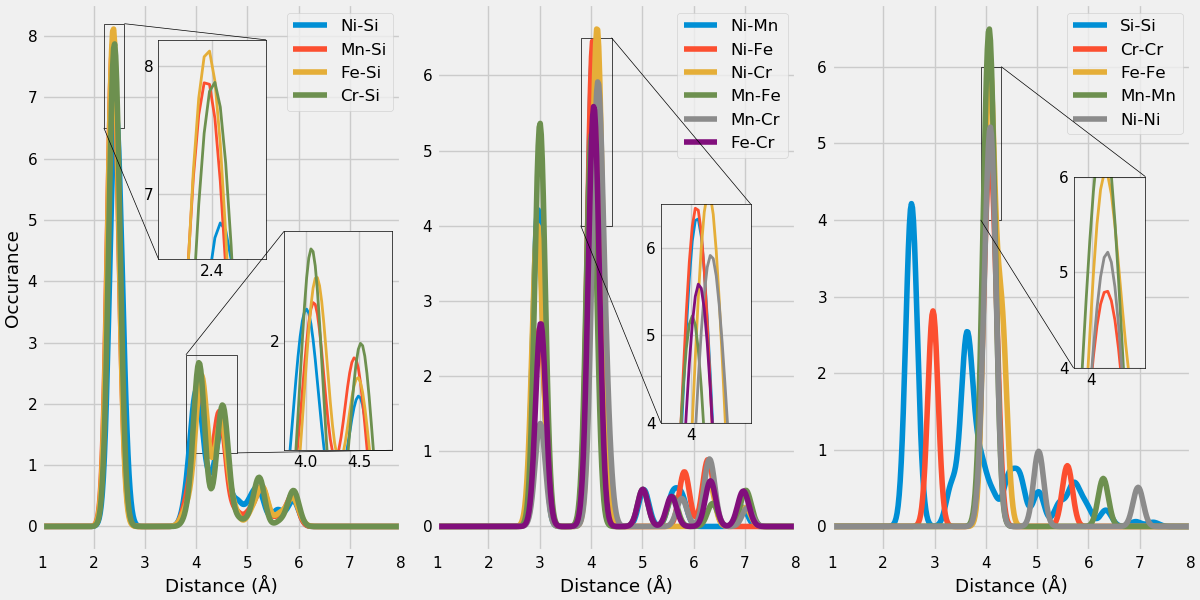
\includegraphics[width=\textwidth]{results/fesi2/D_PDF2.png}
	\end{subfigure}
	\begin{subfigure}{\textwidth}
		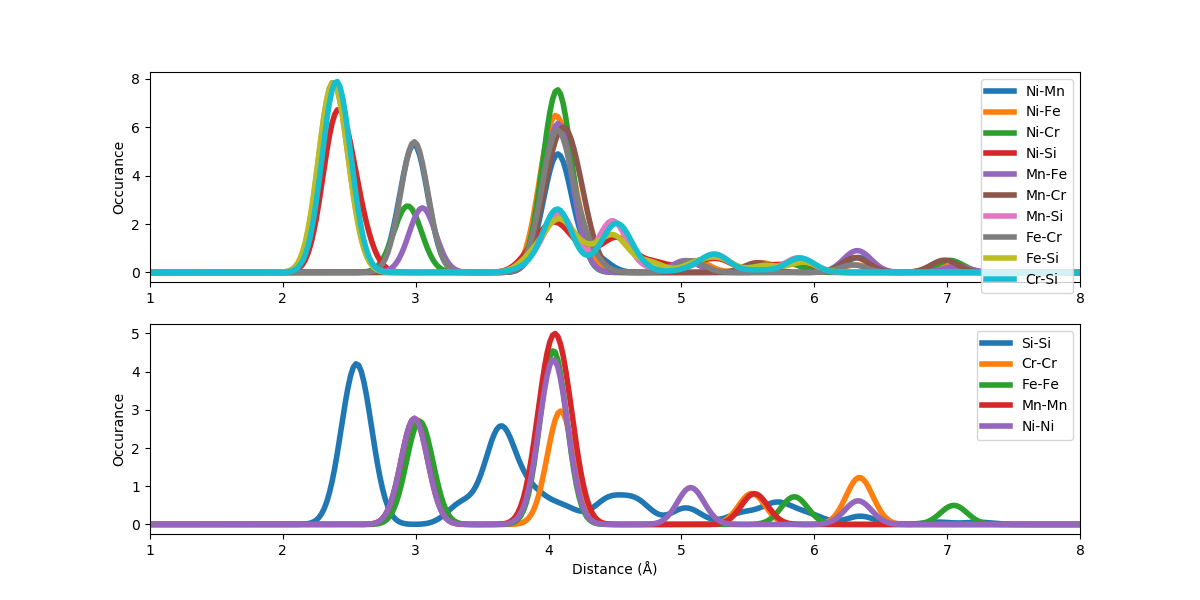
\includegraphics[width=\textwidth]{results/fesi2/B_PDF.png}
	\end{subfigure}
	\caption{Probability distribution function of SQS D (top) and B (bottom)}
\end{figure}

We see that the relative positions of the PDFs remain consistent though both SQSs. With the aid of the ICSD (insert citation), we can compare the figure .. to the expected PDFs based on a number of experiments from a host of different compounds. As our compound contain a total of 15 different bonds, comparing each one to the ICSD values would be an exhaustive process. For our purpose we are satisfied by comparing the 4 different metal-Si bonds. We find that the preferred bond-length of TM-Si is observed at two values, the most dominant being the shorter of the two. For Fe-Si these are between 2.25-2.75 and 4-5, Mn-Si 2.25-2.75 and 3.5-5. Ni-Si lie between 2.25-2.5 and 3.85-5 and Cr-Si between 2.35-2.65 and 4-5.Clearly, the PDFs of the alloys are in good agreement with the listed values for Tm-Si bonds, with the most occurring bond length falling at around 2.4 Å for all TMs, and lesser occurrence between 4.0 - 4.5 Å. The height of the respective peaks is somewhat consistent in both structures, other than slightly reduced Fe-Si occurrence at 2.4 Å in B.

In contrast to the TM-Si bonds, we observe several distinctions between metal bonds in SQS D and B. Covering all would be tedious and not to insightful, instead we emphasize the bonds of Mn and Cr as this is where we found the biggest discrepancy in the PDOS. From the different TM-TM bonds (middle) of figure 8.8 we observe that the Mn-Fe bonds are most occurring at short distances in D and bigger distances in B, meaning that manganese and iron atoms are placed further from each other in structure D. \textbf{correct?} Similarly the bonds between Cr and Fe   indicate that these atoms lie closer in B than D. In contrast the nickel and manganese/chromium bonds point to a closer distance in B for Ni-Mn and Ni-Cr in D, and a greater distance between Ni and Mn in D and Ni and Cr in B. \textbf{Litt kronglete kanskje?} In terms of the homogeneous bonds, the properties of both Cr-Cr bonds and Mn-Mn bonds are more or less alike in both structures besides some majority at shorter distance in D (The red Cr-Cr line at 3Å is underneath the grey Ni-Ni line in B in figure 8.8 (bottom right)). A more significant distinction is that both Ni-Ni and Fe-Fe bonds are found at 3 Å and 4 Å in B, but exclusively 4 Å in D.    

Both the Fe-Fe and Ni-Ni bonds are in better agreement with the ICSD histograms, as the most occurring distance for these bonds are between 4-4.9 Å and additionally around 2.5 Å. \textbf{More comparisons to ICSD, ask O.M}. As a conclusion on the PDFs of this compound, we locate a pattern where the Si-Si bonds are identical and only very minor differences between TM-Si bonds in SQS D and B. This is a result of how the structures are generated with the SQS method. In th FeSi2 structure the silicon atoms are placed as before in the new supercells, but the TM elements are "randomly" distributed. Thus, it's reasonable that also here we would find the major differences between SQSs in the PDFs. 

\newpage
\section{SQS size}
Above we have presented the results of a high-entropy silicide \ch{(CrFeMnNi)Si2} investigated by 5 48 atom SQSs with a volume of $700 Å^3$ before structural relaxations, and found several positive functional properties. This intermediate size allowed for the use of more complex XC-functionals, and secondly enabled a broad study of distinct permutations and compositions. However the application of the special quasi-random structures method to HEAs is not necessarily straightforward. Recalling from section 4.3, the first initial concern is the size of the SQS model and if it's sufficient enough to correctly model the disordered multi-component materials. In this section we will consider this problem by studying the difference between the 48 atom SQS to that of 96 and 192 atom SQS with volume $1200 Å^3$ and $2400 Å^3$ respectively. Below we list the total energy per atom, enthalpy of formation and final magnetic moment in table 7.4, and the band gap in table 7.5 of the respective models, 

\begin{table}[H]
%\centering
\begin{tabular}{@{}cccccc@{}}
\toprule
       & \multicolumn{2}{c}{Total energy/atom (eV)} & Enthalpy of formation (eV) & \multicolumn{2}{c}{Final magnetic moment ($\mu_B$)} \\ \midrule
48 atoms & - 6.6105 & .. & -11.5000 & 0.0833 & 0.0000    \\
96 atoms & - 6.6092  & 0.0021 & - 22.8752  & 0.0708  & 0.0114     \\
192 atoms & - 6.6123  & 0.0022 & - 46.6654 & 0.0761 & 0.0171     \\ \bottomrule
\end{tabular}
\caption{Summary SQS sisze 48, 96, 192 of \ch{(CrFeMnNi)Si2}}
\end{table}

\begin{table}[H]
\centering
\begin{tabular}{@{}ccccc@{}}
\toprule
                                                     &   & Spin up (eV) & Spin down (eV) & Total (eV) \\ \midrule
\multicolumn{1}{c|}{\multirow{5}{*}{\textbf{48 atoms}}}   
												  & A & 0.0815                & 0.0521                  & 0.0281              \\
\multicolumn{1}{c|}{}                                & B & 0.2932                & 0.0523                  & 0.0523              \\
\multicolumn{1}{c|}{}                                & C & 0.2355                & 0.0343                  & 0.0343              \\
\multicolumn{1}{c|}{}                                & \textbf{D} & 0.3386                & 0                       & 0                   \\
\multicolumn{1}{c|}{}                                & E & 0.3078                & 0.0495                  & 0.0495              \\ \midrule
\multicolumn{1}{c|}{\multirow{5}{*}{\textbf{96 atoms}}}   
                                                     & \textbf{A} & 0.1705                & 0.0442                  & 0.0367              \\ 
\multicolumn{1}{c|}{}                                & B & 0.1386                & 0.0270                  & 0.0270                   \\
\multicolumn{1}{c|}{}                                & C & 0.1347                & 0.0363                  & 0.0075                   \\
\multicolumn{1}{c|}{}                                & D & 0.0892                & 0.0398                  & 0.0398                   \\
\multicolumn{1}{c|}{}                                & E & 0.1610                & 0                       & 0                        \\ \midrule
\multicolumn{1}{c|}{\multirow{5}{*}{\textbf{192 atoms}}}
	 									           & A & 0.1197                & 0.0321                  & 0.0321                   \\
\multicolumn{1}{c|}{}                                & B & 0.1444                & 0                       & 0                        \\
\multicolumn{1}{c|}{}                                & C & 0.1867                & 0                       & 0                   \\
\multicolumn{1}{c|}{}                                & D & 0                     & 0                       & 0          \\
\multicolumn{1}{c|}{}                                & \textbf{E} & 0                & 0                       & 0                   \\ \bottomrule
\end{tabular}
\caption{Total and spin dependent band gap of SQS of 48, 96 and 192 atoms each of \ch{(CrFeMnNi)Si2}. The names are arbitrary, ie A in 48 does not equal A in 96 or 192. The most stable SQS is highlighted in bold text.}
\end{table}

As seen from table 7.4 both the total energy and magnetism remain more or less consistent throughout all sizes, this is a good indication of that the 48 atom model can adequately model the alloy. \textbf{Something on the formation enthalpy.} Regarding the band gap, we find that the band gap is lower in the larger cells. In the 48 atom SQSs the gap varies mostly between 0.2 - 0.3 eV. In the 96 model this is reduced to 0.10 - 0.17 eV, and alike in the 192 model. Most instances still point to a spin polarized band gap with larger values in up. A concerning result of this analysis is that it appears that the largest SQS model, attributed by litterture reviews to be the most accurate description to favor a metal, as indicated both by the low number of band gaps in spin up and down compared to the previous cases, and the fact that the most stable configuration have no band gap, as opposed to the smaller cells where the most stable configuration is either half-metallic or semiconducting. However we do see differences between SQSs with some being half-metals and one semiconducting, to draw any real conclusion we should have studied a larger number of SQSs of each size. 

Looking at the pair distribution functions in figure 7.11 we see that the local ordering and short-range interactions is well represented and identical across all three sizes. The distinctions of preferences is largely attributed to the uniqueness of the SQSs more so than the size. On the other hand the larger SQSs clearly provide a better description of large-range interactions, that is not nearly as present in the smaller cell. However as seen in table 7.4 and in accordance with the fundamental concept of the special quasi-random structures method is that the functional properties is mostly determined by short-range effects in the lattice. Therefore, even though the bigger SQSs is a more accurate model the improvement is not justified from the cost, as illustrated in figure 7.12. That is if we neglect the difference of the band gap, which very well could be a product of the uniqeness of the 5 SQSs used in the analysis, or if it's a rigid relevance to the SQS size. \textbf{Something on SQS applied to our case, a XSi2 structure is not really as disordered as a true HEA?}      


\begin{figure}[H]
\begin{subfigure}{\textwidth}
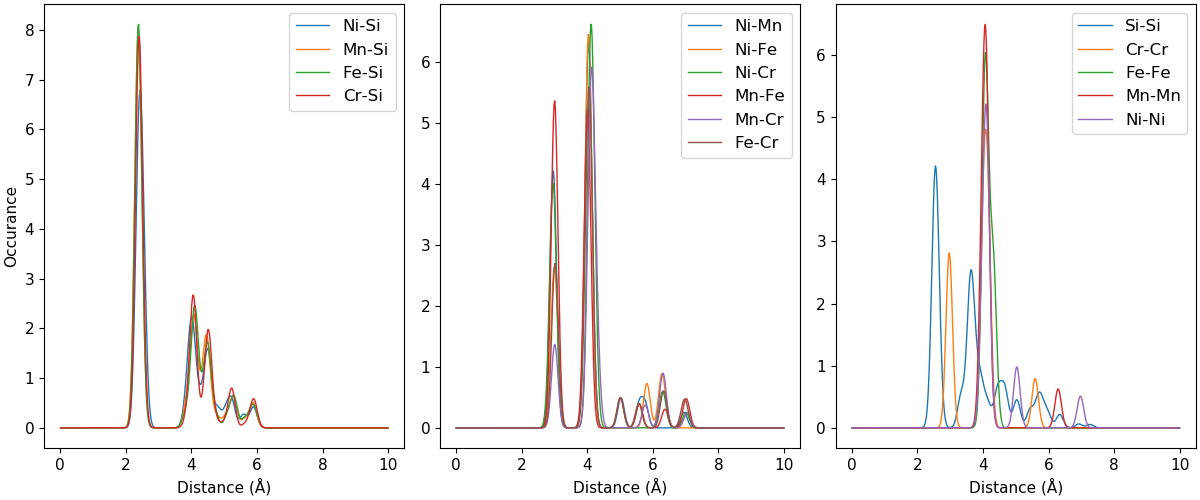
\includegraphics[width=\textwidth]{results/PDF48.png}
\end{subfigure}
\begin{subfigure}{\textwidth}
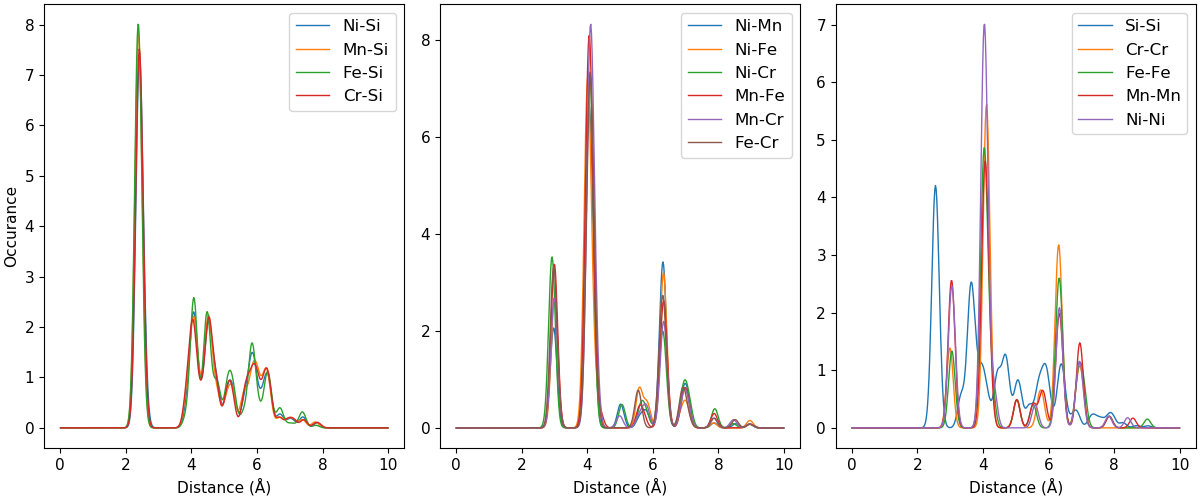
\includegraphics[width=\textwidth]{results/PDF96.png}
\end{subfigure}
\begin{subfigure}{\textwidth}
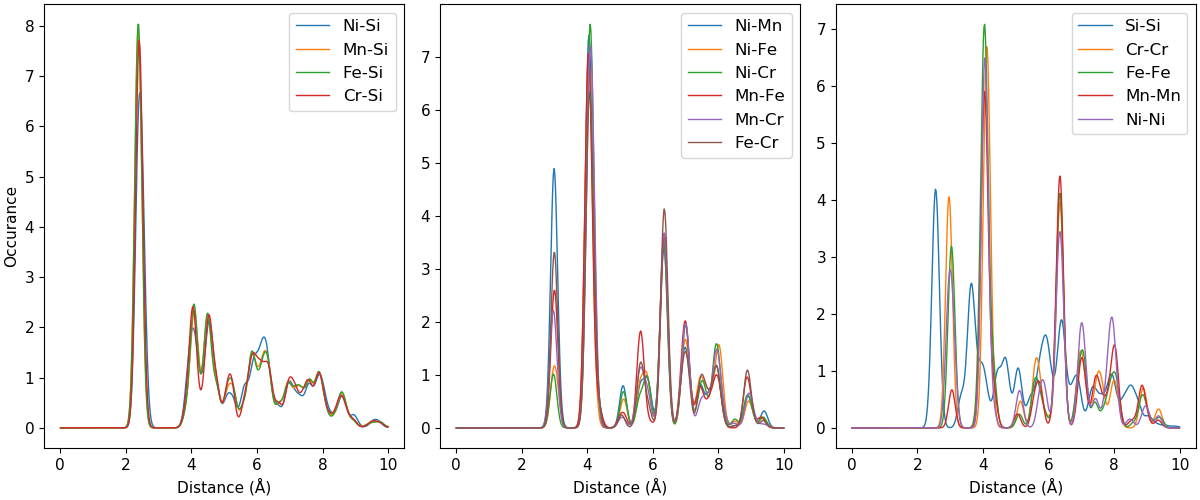
\includegraphics[width=\textwidth]{results/PDF192.png}
\end{subfigure}
\caption{Pair distribution functions of SQS sizes}
\end{figure}


\begin{figure}[H]
\centering
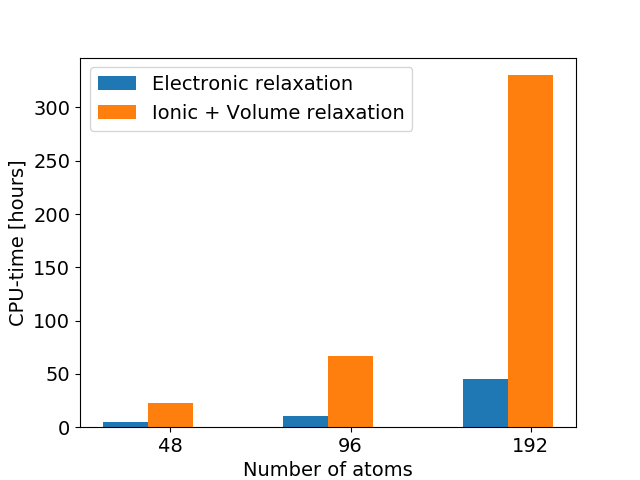
\includegraphics[width=.6\textwidth]{results/SQS_time.png}
\caption{CPU time}
\end{figure}


